\documentclass[11pt, a4paper]{article}
\usepackage[margin=2.4cm]{geometry}
\usepackage[T1]{fontenc}
\usepackage{lmodern}          % fontes vetoriais Type 1
\usepackage{cmap}             % ToUnicode CMap -> texto e acentos copiaveis
\usepackage[utf8]{inputenc}
\usepackage[brazil]{babel}
\usepackage{amsmath, amssymb, amsthm}
\usepackage{bm}
\usepackage{mathtools}
\usepackage{enumitem}
\usepackage{booktabs}
\usepackage{array}
\usepackage{xcolor}
\usepackage{titlesec}
\usepackage{parskip}
\usepackage{hyperref}
\usepackage{fancyhdr}
\usepackage{tcolorbox}
\usepackage{graphicx}
\usepackage{pgfplots}
\pgfplotsset{compat=1.18}
\usetikzlibrary{arrows.meta, decorations.pathreplacing}
\tcbuselibrary{skins, breakable}

\definecolor{darkblue}{RGB}{15,55,115}
\definecolor{midblue}{RGB}{30,100,180}
\definecolor{theorybg}{RGB}{245,250,255}
\definecolor{questionbg}{RGB}{255,252,240}
\definecolor{evencolor}{RGB}{60,0,100}
\definecolor{rubricbg}{RGB}{248,246,252}

\hypersetup{colorlinks=true, linkcolor=darkblue, urlcolor=midblue,
  pdftitle={Resolucao --- Lista de Exercicios 1 --- Macroeconomia I MPE Insper},
  pdfauthor={Macroeconomia I --- MPE Insper 2026/T3}}

\setlength{\headheight}{14pt}
\pagestyle{fancy}
\fancyhf{}
\renewcommand{\headrulewidth}{0.4pt}
\fancyhead[L]{\small\textcolor{darkblue}{\textit{Macroeconomia I --- MPE Insper --- 2026/T3}}}
\fancyhead[R]{\small\textcolor{darkblue}{\thepage}}
\fancyfoot[C]{\small\textcolor{gray}{Resolução --- Lista de Exercícios 1}}

\titleformat{\section}[block]
  {\large\bfseries\color{darkblue}}{}{0pt}{}
  [\vspace{2pt}\color{darkblue}\rule{\textwidth}{1.5pt}\vspace{4pt}]

\tcbset{
  theorybox/.style={
    enhanced, breakable, colback=theorybg, colframe=darkblue,
    fonttitle=\bfseries\small, coltitle=white, boxrule=0.5pt, arc=3pt,
    left=6pt, right=6pt, top=4pt, bottom=4pt,
  },
  questionbox/.style={
    enhanced, breakable, colback=questionbg, colframe=gray!60,
    fonttitle=\bfseries\small, coltitle=black, boxrule=0.4pt, arc=2pt,
    left=6pt, right=6pt, top=4pt, bottom=4pt, title={\textit{Enunciado}},
  },
  rubricbox/.style={
    enhanced, breakable, colback=rubricbg, colframe=evencolor!70,
    fonttitle=\bfseries\small, coltitle=white, boxrule=0.4pt, arc=2pt,
    left=6pt, right=6pt, top=4pt, bottom=4pt, title={Onde estão os pontos},
  },
  oddbox/.style={
    enhanced, breakable, colback=white, colframe=darkblue,
    attach boxed title to top left={yshift=-2mm, xshift=6mm},
    boxed title style={colback=darkblue, colframe=darkblue, arc=2pt,
      boxrule=0pt, left=6pt, right=6pt, top=3pt, bottom=3pt},
    fonttitle=\bfseries\large\color{white},
    boxrule=0.8pt, arc=3pt, left=8pt, right=8pt, top=10pt, bottom=6pt,
  },
  evenbox/.style={
    enhanced, breakable, colback=white, colframe=evencolor,
    attach boxed title to top left={yshift=-2mm, xshift=6mm},
    boxed title style={colback=evencolor, colframe=evencolor, arc=2pt,
      boxrule=0pt, left=6pt, right=6pt, top=3pt, bottom=3pt},
    fonttitle=\bfseries\large\color{white},
    boxrule=0.8pt, arc=3pt, left=8pt, right=8pt, top=10pt, bottom=6pt,
  },
}

\newcommand{\passo}[1]{\medskip\noindent\textbf{#1}\par\nobreak}
\newcommand{\intuicao}[1]{%
  \medskip\noindent\textcolor{midblue}{\textbf{Intuição econômica.}} #1\par}
\newcommand{\refbib}[1]{%
  \medskip\noindent{\small\textcolor{gray!60!black}{\textbf{Ref:} #1}}\par}
\newcommand{\resp}[1]{\textcolor{darkblue}{\textbf{#1}}}
\newcommand{\stst}{^{\ast}}
\newcommand{\ststst}{^{\ast\ast}}
\DeclareMathOperator{\Cov}{Cov}

\setlist[enumerate,1]{label=(\alph*), itemsep=6pt, parsep=2pt, leftmargin=1.6em}
\setlist[itemize,1]{itemsep=3pt, parsep=1pt, leftmargin=1.3em, topsep=3pt}

\begin{document}

%======================================================================
\begin{center}
{\LARGE\bfseries\color{darkblue} Resolução --- Lista de Exercícios 1\par}
\vspace{4pt}
{\large MACROECONOMIA 1 --- MPE Insper --- Prof.\ Pedro G.\ Duarte\par}
\vspace{2pt}
{\normalsize 2026, 3\textordmasculine{} trimestre \quad$\cdot$\quad Entrega: 10/8, 19h30\par}
\end{center}
\vspace{6pt}

\begin{tcolorbox}[theorybox, title={Como ler este documento}]
\small
Quatro questões, 10 pontos. As Questões 1 e 4 são de papel e caneta; a Questão 2 é
discursiva; a \textbf{Questão 3 é um exercício de dados} --- exige baixar a Penn World
Table e produzir gráficos. Aqui ela está resolvida com dados de verdade (PWT 10.01),
não apenas com o padrão esperado.

\smallskip
\textbf{Verificação.} Todo número deste documento foi calculado em Python; os scripts
estão em \texttt{Resolucao/lista1\_codigo/} e listados no Apêndice. As contas
da Questão 1 usam aritmética de frações exatas (\texttt{fractions.Fraction}), e os
resultados da Questão 4 conferem a fórmula analítica contra a simulação numérica. Onde
aparece \checkmark, o resultado foi checado por um segundo caminho independente.

\smallskip
\textbf{Escopo.} Tudo se apoia em Kurlat (2020), caps.\ 1--4. Nenhum instrumento fora do
programa foi usado. Referências de página são da edição em \texttt{Livros/}
(Kurlat: página impressa $=$ página do PDF).
\end{tcolorbox}

\vspace{4pt}
\begin{center}
\small
\begin{tabular}{clcl}
\toprule
\textbf{Questão} & \textbf{Assunto} & \textbf{Pontos} & \textbf{Âncora} \\
\midrule
1 & PIB nominal, real, números-índice e PPC & 3,0 (0,6/item) & Kurlat cap.\ 1 (pp.\ 15--26) \\
2 & Bem-estar além do PIB (Exercício 2.2)   & 2,0            & Kurlat cap.\ 2 (pp.\ 31--39) \\
3 & Convergência dentro de regiões (Ex.\ 3.3) & 2,0          & Kurlat §3.3 (p.\ 51) \\
4 & Terremoto no modelo de Solow            & 3,0 (1,5/item) & Kurlat §4.1--4.2 (pp.\ 53--60) \\
\bottomrule
\end{tabular}
\end{center}

%======================================================================
\section[Questão 1 --- PIB nominal, PIB real e comparações internacionais]{Questão 1 \quad PIB nominal, PIB real e comparações internacionais \hfill \normalsize (3 pontos)}
%======================================================================

\begin{tcolorbox}[questionbox]
\small
Baseado em Kurlat (2020, Cap.\ 1). Preços (em reais) e quantidades dos bens 1 e 2
produzidos no \textbf{Brasil}:

\begin{center}
\begin{tabular}{ccccc}
\toprule
 & $p_1$ & $q_1$ & $p_2$ & $q_2$ \\
\midrule
2024 & 8 & 5  & 4 & 4 \\
2025 & 2 & 12 & 6 & 3 \\
\bottomrule
\end{tabular}
\end{center}

\textbf{(a)} PIB nominal em 2024 e 2025. \textbf{(b)} PIB real de 2025 a preços de 2024 e a
taxa de crescimento. \textbf{(c)} PIB real de 2024 a preços de 2025 e a taxa de crescimento;
o que explica a diferença para o item anterior?

Na \textbf{Colômbia}, preços (em pesos colombianos) e quantidades em 2024:

\begin{center}
\begin{tabular}{ccccc}
\toprule
 & $p_1$ & $q_1$ & $p_2$ & $q_2$ \\
\midrule
2024 & 40 & 1 & 8 & 2 \\
\bottomrule
\end{tabular}
\end{center}

\textbf{(d)} Com câmbio de 25 pesos por 1 real, o PIB colombiano de 2024 em reais à taxa de
mercado. \textbf{(e)} O PIB colombiano de 2024 à paridade do poder de compra (PPC); o que
explica a diferença entre os dois valores?
\end{tcolorbox}

\passo{Método.} Toda a questão é uma aplicação de uma única definição --- o PIB é
$\sum_i p_i q_i$ --- com a pergunta \emph{a qual vetor de preços} avaliar as quantidades.
Nos itens (a)--(c) a escolha é entre dois \textbf{anos}; nos itens (d)--(e), entre dois
\textbf{países}. É o mesmo problema de número-índice nas duas metades, e vale enxergá-lo
assim desde o começo: é isso que a questão está testando.

%---------------------------------------------------------------- (a)
\subsection*{(a) PIB nominal brasileiro}

O PIB nominal avalia as quantidades de cada ano aos preços \emph{daquele mesmo} ano:
$$\text{PIB}^{\text{nom}}_t \;=\; \sum_i p_{i,t}\, q_{i,t}.$$

\begin{align*}
\text{PIB}^{\text{nom}}_{2024} &= (8)(5) + (4)(4) = 40 + 16 = \resp{56 \text{ reais}},\\[2pt]
\text{PIB}^{\text{nom}}_{2025} &= (2)(12) + (6)(3) = 24 + 18 = \resp{42 \text{ reais}}.
\end{align*}

\passo{Observação que já antecipa (b) e (c).} O PIB nominal \textbf{caiu} 25\%
($42/56 - 1 = -0{,}25$). Seria um erro grave concluir daí que a economia encolheu: as
duas quantidades produzidas não caíram juntas --- o bem 1 mais que dobrou
($5 \to 12$) --- e o que derrubou o valor nominal foi o colapso do preço do bem 1
($8 \to 2$). Separar preço de quantidade é exatamente o que os itens seguintes fazem.

%---------------------------------------------------------------- (b)
\subsection*{(b) PIB real a preços de 2024 (ano-base 2024)}

Fixe o vetor de preços em $p_{2024} = (8,4)$ e avalie as quantidades dos dois anos:

\begin{align*}
\text{PIB}^{\text{real}}_{2024}\big|_{p_{2024}} &= (8)(5) + (4)(4) = \resp{56 \text{ reais}}
  \quad (\text{no ano-base, real} = \text{nominal}),\\[2pt]
\text{PIB}^{\text{real}}_{2025}\big|_{p_{2024}} &= (8)(12) + (4)(3) = 96 + 12 = \resp{108 \text{ reais}}.
\end{align*}

Taxa de crescimento:
$$g^{L} \;=\; \frac{108}{56} - 1 \;=\; \frac{52}{56} \;=\; \frac{13}{14} \;=\;
\resp{+92{,}86\%}.$$

Este é um índice de quantidade de \textbf{Laspeyres} (pesos do ano-base):
$Q^{L} = \dfrac{\sum_i p_{i,0}\, q_{i,1}}{\sum_i p_{i,0}\, q_{i,0}} = 1{,}9286$.

%---------------------------------------------------------------- (c)
\subsection*{(c) PIB real a preços de 2025 (ano-base 2025) e a origem da diferença}

Agora fixe $p_{2025} = (2,6)$:

\begin{align*}
\text{PIB}^{\text{real}}_{2024}\big|_{p_{2025}} &= (2)(5) + (6)(4) = 10 + 24 = \resp{34 \text{ reais}},\\[2pt]
\text{PIB}^{\text{real}}_{2025}\big|_{p_{2025}} &= (2)(12) + (6)(3) = \resp{42 \text{ reais}}
  \quad (= \text{nominal de 2025}).
\end{align*}

$$g^{P} \;=\; \frac{42}{34} - 1 \;=\; \frac{8}{34} \;=\; \frac{4}{17} \;=\; \resp{+23{,}53\%}.$$

Este é um índice de quantidade de \textbf{Paasche} (pesos do ano corrente):
$Q^{P} = \dfrac{\sum_i p_{i,1}\, q_{i,1}}{\sum_i p_{i,1}\, q_{i,0}} = 1{,}2353$.

\passo{Por que $92{,}86\%$ e $23{,}53\%$?} A diferença não é erro de conta nem detalhe
técnico: \textbf{os preços relativos mudaram, e mudaram na direção oposta às
quantidades.}

\begin{center}
\begin{tabular}{lccc}
\toprule
 & \begin{tabular}{@{}c@{}}relativo de preço\\ $r_i = p_{i,1}/p_{i,0}$\end{tabular}
 & \begin{tabular}{@{}c@{}}relativo de quantidade\\ $s_i = q_{i,1}/q_{i,0}$\end{tabular}
 & \begin{tabular}{@{}c@{}}peso em 2024\\ $w_i$\end{tabular} \\
\midrule
Bem 1 & $2/8 = 0{,}25$ & $12/5 = 2{,}40$ & $40/56 = 0{,}714$ \\
Bem 2 & $6/4 = 1{,}50$ & $3/4  = 0{,}75$ & $16/56 = 0{,}286$ \\
\bottomrule
\end{tabular}
\end{center}

O bem que \emph{barateou} foi o que mais \emph{cresceu}. Então:

\begin{itemize}
\item Avaliando a preços de \textbf{2024}, o bem 1 ainda vale 8 --- é o bem caro,
      carrega peso $0{,}714$ --- e é justamente ele que dispara. O índice pega peso grande
      $\times$ crescimento grande e devolve $+92{,}86\%$.
\item Avaliando a preços de \textbf{2025}, o bem 1 vale 2 --- virou o bem barato. Seu
      crescimento passa a contar pouco, e o índice cai para $+23{,}53\%$.
\end{itemize}

\passo{A conta que formaliza isso (identidade de Bortkiewicz).} Escrevendo os índices como
médias ponderadas dos relativos, com pesos $w_i$ do ano-base,
$$P^{L} = \sum_i w_i r_i, \qquad Q^{L} = \sum_i w_i s_i, \qquad
\frac{V_1}{V_0} = \sum_i w_i r_i s_i,$$
onde $V_t$ é o PIB nominal. Como $Q^{P} = (V_1/V_0)/P^{L}$, divide-se um pelo outro:
$$\boxed{\;\frac{Q^{P}}{Q^{L}} \;=\;
\frac{\sum_i w_i r_i s_i}{\left(\sum_i w_i r_i\right)\left(\sum_i w_i s_i\right)}
\;=\; 1 + \frac{\Cov_w(r,s)}{P^{L}\, Q^{L}}\;}$$

Numericamente:
$$\Cov_w(r,s) = 0{,}75 - (0{,}6071)(1{,}9286) = -0{,}4209
\;\Longrightarrow\;
\frac{Q^{P}}{Q^{L}} = 1 - \frac{0{,}4209}{1{,}1709} = 0{,}6405,$$
e, de fato, $1{,}2353/1{,}9286 = 0{,}6405$. \checkmark

A leitura é limpa: \textbf{sempre que preços e quantidades se movem em direções opostas
(substituição), a covariância é negativa e Paasche fica abaixo de Laspeyres.} Não é uma
coincidência deste exercício --- é o \emph{viés de substituição}, a razão pela qual um
índice de Laspeyres (como o IPCA, de cesta fixa) superestima a inflação e um índice de
Paasche a subestima.

\passo{O que os órgãos estatísticos fazem: encadeamento.} Não se escolhe entre os dois
--- toma-se a média geométrica, o índice de \textbf{Fisher}:
$$Q^{F} = \sqrt{Q^{L}\, Q^{P}} = \sqrt{(1{,}9286)(1{,}2353)} = 1{,}5435
\;\Longrightarrow\; g^{F} = \resp{+54{,}35\%},$$
$$P^{F} = \sqrt{P^{L}\, P^{P}} = \sqrt{(0{,}6071)(0{,}3889)} = 0{,}4859
\;\Longrightarrow\; \pi^{F} = -51{,}41\%.$$

\emph{Teste de consistência (o "product test"):} preço $\times$ quantidade tem de reproduzir
o valor nominal. $P^{F} \cdot Q^{F} = 0{,}4859 \times 1{,}5435 = 0{,}7500 = 42/56$.
\checkmark\ É esse encadeamento que o IBGE e o BEA usam, e é por isso que o ano-base
deixou de aparecer nas contas nacionais modernas.

\emph{Deflator implícito:} com base 2024 $=100$, o deflator de 2025 é
$100 \times 42/108 = 38{,}89$ --- ou seja, o índice de Paasche de preços. Note que o
deflator do PIB \emph{é}, por construção, um índice de Paasche; o IPCA é de Laspeyres.
Essa é a diferença conceitual entre os dois, e ela aparece inteira neste exercício.

%---------------------------------------------------------------- (d)
\subsection*{(d) PIB colombiano à taxa de câmbio de mercado}

Primeiro, em moeda local:
$$\text{PIB}^{\text{COL}}_{2024} = (40)(1) + (8)(2) = 40 + 16 = 56 \text{ pesos}.$$

Convertendo à taxa de mercado $e = 25$ pesos por real:
$$\text{PIB}^{\text{COL}}_{\text{câmbio}} = \frac{56}{25} = \resp{2{,}24 \text{ reais}}.$$

Comparado ao Brasil ($56$ reais), isso faria a Colômbia valer \textbf{4,0\%} do PIB
brasileiro.

%---------------------------------------------------------------- (e)
\subsection*{(e) PIB colombiano a PPC}

À paridade do poder de compra, avaliam-se as \emph{quantidades colombianas} a um vetor de
preços comum. Tomando os preços brasileiros de 2024 como numerário:
$$\text{PIB}^{\text{COL}}_{\text{PPC}} = \sum_i p^{\text{BRA}}_{i,2024}\, q^{\text{COL}}_{i,2024}
= (8)(1) + (4)(2) = 8 + 8 = \resp{16 \text{ reais}}.$$

Agora a Colômbia vale \textbf{28,6\%} do PIB brasileiro --- \resp{$7{,}14$ vezes} o que a
conversão pelo câmbio de mercado indicava.

\passo{O que explica a diferença.} A taxa de câmbio de mercado \emph{não} iguala o poder
de compra das duas moedas. A taxa de câmbio PPC implícita é
$$e^{\text{PPC}} = \frac{\text{PIB em pesos}}{\text{PIB em reais a preços do Brasil}}
= \frac{56}{16} = 3{,}5 \text{ pesos por real},$$
contra $25$ pesos por real no mercado. O nível de preços colombiano é, portanto, cerca de
$3{,}5/25 = 14\%$ do brasileiro: \textbf{tudo é barato na Colômbia quando medido em
reais}. Converter pelo câmbio de mercado trata esse barateamento como se fosse
\emph{menos produto}, quando na verdade é \emph{o mesmo produto a preços menores}.

Economicamente, a razão é que a taxa de câmbio de mercado é determinada sobretudo pelos
bens \textbf{comercializáveis} e pelos fluxos financeiros, ao passo que boa parte do PIB
é composta de \textbf{não-comercializáveis} (serviços, aluguel, transporte local) --- e
esses são sistematicamente mais baratos em países mais pobres, porque o salário é mais
baixo e eles são intensivos em trabalho. É o efeito \textbf{Balassa--Samuelson}, e é a
razão de existir a Penn World Table.

\passo{O mesmo problema de número-índice de novo --- agora entre países.} Note que a
escolha do vetor de preços é tão arbitrária aqui quanto era em (b)--(c). Se avaliássemos
as duas economias a preços \emph{colombianos}, a cesta brasileira valeria
$(40)(5)+(8)(4) = 232$ pesos, e a Colômbia seria $56/232 = 24{,}1\%$ do Brasil --- não
$28{,}6\%$. A média geométrica das duas dá $\sqrt{(0{,}2857)(0{,}2414)} = 26{,}3\%$, e o
câmbio PPC de Fisher é $\sqrt{(3{,}5)(4{,}143)} = 3{,}81$ pesos por real.

E a origem da discrepância é a mesma de antes: os \textbf{preços relativos diferem entre
os países}. No Brasil $p_1/p_2 = 2$; na Colômbia $p_1/p_2 = 5$. O bem 1 é relativamente
caro na Colômbia --- e é justamente dele que os colombianos produzem pouco
($q_1 = 1$ contra $q_2 = 2$). Substituição de novo, só que no espaço em vez do tempo. É
por isso que a PWT usa métodos multilaterais (Geary--Khamis, EKS) em vez de escolher um
país-base.

\intuicao{Os cinco itens contam uma história só. Um número de PIB só significa alguma
coisa depois que se responde ``a que preços?''. Quando os preços relativos se mexem --- e
eles sempre se mexem, seja entre 2024 e 2025, seja entre Brasil e Colômbia --- não existe
resposta única, existe uma \emph{faixa} delimitada por Laspeyres e Paasche. O encadeamento
de Fisher é a convenção que resolve o impasse, e o faz porque satisfaz o teste do produto.
Quem responde (b) e (c) com dois números sem explicar que ambos estão corretos perdeu a
questão.}

\refbib{Kurlat (2020), cap.\ 1 --- §1.1 ``GDP Accounting'' (p.\ 15) para a definição, e
§1.2 ``Making Comparisons'' (pp.\ 22--26) para números-índice, encadeamento e PPC. Para
os dados e o contraste institucional, Jones (2020, 5\textordfeminine{} ed.), cap.\ 2.}

\begin{tcolorbox}[rubricbox]
\small
\textbf{(a)} 0,6 --- os dois números. \textbf{(b)} 0,6 --- PIB real (0,3) $+$ taxa (0,3).
\textbf{(c)} 0,6 --- números (0,3) $+$ \emph{explicação} da divergência (0,3).
\textbf{(d)} 0,6. \textbf{(e)} 0,6 --- valor PPC (0,3) $+$ explicação (0,3).

\smallskip
\textbf{Tetos por erro conceitual} (prevalecem sobre penalidades leves, não se somam):
\begin{itemize}[topsep=2pt]
\item Dizer que o PIB real de 2024 a preços de 2024 é diferente de 56 (não entendeu que no
      ano-base real $=$ nominal): máx.\ 0,3 no item.
\item Afirmar que uma das taxas de (b)/(c) está ``errada'' e a outra ``certa'': máx.\ 0,3
      em (c). \emph{As duas estão corretas} --- respondem a perguntas diferentes.
\item Em (e), converter os pesos pela taxa de mercado em vez de reavaliar as quantidades
      a preços comuns (isto é, repetir o item (d)): 0 no item.
\item Justificar (e) só com ``a moeda está desvalorizada'', sem falar em preços de
      não-comercializáveis ou nível de preços: máx.\ 0,3.
\end{itemize}
\textbf{Penalidade leve:} erro aritmético com método visivelmente correto, $-0{,}1$.
\end{tcolorbox}

%======================================================================
\section[Questão 2 --- Bem-estar além do PIB (Kurlat 2.2)]{Questão 2 \quad Bem-estar além do PIB --- Kurlat, Exercício 2.2 \hfill \normalsize (2 pontos)}
%======================================================================

\begin{tcolorbox}[questionbox]
\small
A medida de bem-estar $\lambda$ leva em conta dados de consumo, desigualdade, lazer e
mortalidade.

\textbf{(a)} Cite uma outra variável que possa ser determinante importante do bem-estar e
que não esteja incluída no cálculo usual do PIB.

\textbf{(b)} De que dados você precisaria para descobrir quanto peso dar a essa variável?
Descreva como usaria esses dados para chegar à forma correta de incluí-la no cálculo de
bem-estar. Que escolhas que as pessoas fazem revelariam o quanto elas se importam com essa
variável? Não se preocupe muito com a viabilidade da coleta, mas pense com cuidado sobre
\emph{por que} as escolhas observadas seriam informativas.
\end{tcolorbox}

\begin{tcolorbox}[theorybox, title={Onde está o peso da questão}]
\small
O item (a) vale pouco: qualquer variável defensável serve. \textbf{O que está sendo
avaliado é a lógica de preferência revelada do item (b)} --- por que uma escolha
observada carrega informação sobre uma valoração que ninguém declara. Escreva pouco em
(a) e muito em (b).
\end{tcolorbox}

%---------------------------------------------------------------- (a)
\subsection*{(a) A variável: segurança pessoal (risco de ser vítima de crime violento)}

\resp{Proponho a segurança pessoal} --- concretamente, o risco de ser vítima de homicídio
ou de crime violento.

Três razões para preferi-la a outras candidatas:

\begin{itemize}
\item \textbf{É grande.} No Brasil, a taxa de homicídios varia de menos de 10 por 100 mil
      habitantes em alguns estados a mais de 50 em outros. A renda per capita não varia
      nem de longe nessa proporção. Uma variável que se move muito mais do que a renda
      pode mudar materialmente uma comparação de bem-estar.
\item \textbf{O PIB a trata de forma perversa.} Gasto com grades, seguro, alarme,
      segurança privada e reposição de bens roubados \textbf{entra} no PIB. Um país mais
      violento pode, por isso, parecer \emph{mais rico}. O sinal está literalmente
      invertido em relação ao bem-estar --- é um exemplo particularmente limpo do
      argumento do cap.\ 2 de Kurlat.
\item \textbf{É estimável.} Como se verá em (b), a identificação exige variação da
      variável que não venha acompanhada de tudo mais. Criminalidade oferece essa variação
      --- geograficamente fina e com mudanças de política discretas no tempo.
\end{itemize}

Outras respostas igualmente defensáveis: qualidade do ar, tempo de deslocamento casa--%
trabalho, liberdade política e civil, estabilidade no emprego, qualidade das relações
sociais. \emph{Qualquer uma serve, desde que em (b) você consiga descrever uma escolha
observável que a precifique.} É esse o critério, e é por isso que ``felicidade'' é uma
resposta fraca: não há escolha que a revele contra dinheiro.

%---------------------------------------------------------------- (b)
\subsection*{(b) Como precificar: dados, método e por que a escolha é informativa}

\passo{Passo 1 --- Por que não perguntar.} A rota óbvia --- uma pesquisa perguntando
``quanto você pagaria para viver em um bairro seguro?'' --- é a rota ruim. Isso é
\textbf{preferência declarada}, e as respostas não têm consequência: quem responde não
paga nada por exagerar. O viés hipotético é grande e sistemático. A alternativa é a
\textbf{preferência revelada}: procurar uma decisão real, custosa e repetida em que a
pessoa troque a variável por dinheiro. O preço implícito nessa troca é o peso que se
procura.

\passo{Passo 2 --- Método 1: preços hedônicos de moradia (o cavalo de batalha).}

\emph{Dados necessários:} microdados de aluguéis ou preços de venda de imóveis com
localização precisa (CEP ou setor censitário); taxas de criminalidade na mesma
granularidade geográfica (no Brasil, boletins de ocorrência das Secretarias de Segurança e
o Sistema de Informações sobre Mortalidade do Ministério da Saúde para homicídios);
atributos do imóvel (área, idade, número de quartos, vaga) e do entorno (qualidade das
escolas, distância ao centro de emprego, transporte, comércio).

\emph{Estimação:}
$$\ln(\text{aluguel}_i) = \beta_0 + \beta_1\,\text{crime}_i + \gamma' X_i + \varepsilon_i,$$
em que $X_i$ recolhe todos os atributos observáveis. O coeficiente $-\beta_1$ é a
\textbf{disposição marginal a pagar} por uma unidade de redução do risco, expressa como
fração do custo de moradia.

\emph{Por que isso é informativo:} escolher onde morar é uma decisão real, cara, difícil
de reverter e que a família revisita ao longo de anos. Quem aceita pagar mais caro por um
apartamento idêntico num bairro mais seguro está literalmente convertendo segurança em
reais, e tem todo o incentivo de acertar a conta. O diferencial de aluguel
\textbf{capitaliza} a diferença de segurança.

\emph{O problema de identificação, e o conserto.} Bairro violento é também bairro com
escola pior, menos infraestrutura e menos serviço público. Numa regressão de corte
transversal, $\beta_1$ capta tudo isso junto e superestima o valor da segurança. É preciso
variação em criminalidade que seja \textbf{ortogonal} ao resto:
\begin{itemize}
\item uma reforma de policiamento implantada em alguns distritos e não em outros
      (a instalação escalonada das UPPs no Rio é o exemplo brasileiro canônico);
\item comparar aluguéis \textbf{dentro do mesmo bairro, antes e depois} da intervenção,
      contra bairros parecidos que não a receberam --- diferenças-em-diferenças, que
      elimina tudo o que é fixo no bairro.
\end{itemize}
Sem uma fonte de variação assim, o número estimado não é o peso que se quer.

\passo{Passo 3 --- Método 2: diferenciais compensatórios de salário.}

Ocupações mais perigosas pagam mais, tudo o mais constante. Regredindo salário sobre risco
de morte no trabalho, controlando por escolaridade, experiência e setor, obtém-se o prêmio
salarial por unidade de risco de mortalidade e, dele, o \textbf{valor de uma vida
estatística} (VSL). A lógica é idêntica à do método 1 --- o trabalhador troca dinheiro por
risco --- e tem a vantagem de já ser a mesma técnica que Jones e Klenow usam para
precificar expectativa de vida. Ou seja, ela \emph{encaixa} no arcabouço, em vez de
precisar ser costurada nele.

\passo{Passo 4 --- Método 3: migração.} Quem deixa uma região violenta aceitando um
emprego pior em outra revela um limite inferior para o que está disposto a pagar por
segurança: o salário abandonado. É um método mais grosseiro (migrar tem custos fixos que
contaminam o cálculo), mas serve de checagem de ordem de grandeza para os dois anteriores.

\passo{Passo 5 --- Como colocar no cálculo de bem-estar.} A utilidade de fluxo de Jones e
Klenow ganha um argumento de segurança $s$:
$$u(c, \ell, a, s) = \left[\bar u + \frac{c^{1-\sigma}}{1-\sigma} - \theta\,\frac{(1-\ell)^{1+\phi}}{1+\phi}
+ \psi\, v(s)\right] a .$$
Calibra-se $\psi$ impondo que a taxa marginal de substituição do modelo reproduza a
estimada no passo 2:
$$\underbrace{\frac{\partial u/\partial s}{\partial u/\partial c}}_{\text{modelo}}
\;=\;
\underbrace{\text{DAP por unidade de segurança}}_{\text{regressão hedônica}} .$$
Com $\psi$ na mão, recalcula-se $\lambda$ país a país. Países mais seguros que os EUA têm
$\lambda$ revisado \textbf{para cima}; o Brasil, com taxa de homicídios muitas vezes a
americana, seria revisado \textbf{para baixo}.

\passo{Passo 6 --- A ressalva que separa uma resposta boa de uma resposta completa.} Se o
crime mata, parte do seu custo \textbf{já está contabilizada} via expectativa de vida $a$,
que a medida $\lambda$ já inclui. Somar $\psi v(s)$ por cima seria \textbf{dupla
contagem}. O termo de segurança precisa ser calibrado sobre a parcela que \emph{não}
aparece na mortalidade: o medo, o comportamento defensivo (não sair à noite, não usar
certo trajeto, não portar celular), a vitimização não-fatal e o gasto privado com
proteção. Na prática, isso significa estimar o passo 2 usando crime \emph{contra o
patrimônio} ou vitimização não-letal, e não homicídios.

\intuicao{A ideia central do cap.\ 2 é que ``o que não está no PIB'' não é uma lista de
lamentos --- é um problema de mensuração com solução. Se uma variável afeta o bem-estar,
ela afeta escolhas; se afeta escolhas, ela tem um preço-sombra; e se tem preço-sombra, ela
pode entrar na função de utilidade com um peso disciplinado por dados em vez de
arbitrado. É a mesma lógica que permite a Jones e Klenow pôr lazer, desigualdade e
mortalidade na mesma unidade de conta que o consumo. A pergunta não é ``o PIB é uma medida
imperfeita?'' --- todo mundo concorda que é --- mas ``consegue-se corrigi-la de forma
disciplinada?''.}

\refbib{Kurlat (2020), cap.\ 2 --- §2.1 ``The Human Development Index'' (p.\ 31) e §2.2
``Beyond GDP'' (pp.\ 33--39), onde a medida $\lambda$ de Jones--Klenow é construída;
enunciado do Exercício 2.2 na p.\ 40. Para o método de preferência revelada aplicado a
mortalidade, ver a discussão do valor da vida em §2.2.}

\begin{tcolorbox}[rubricbox]
\small
\textbf{(a)} 0,5 --- variável plausível e fora do PIB (0,3); justificar por que importa
\emph{e} por que o PIB não a capta (0,2).
\textbf{(b)} 1,5 --- identificar a lógica de \textbf{preferência revelada} (0,5);
descrever \emph{um} método concreto com os dados de que precisa (0,5); explicar por que a
escolha observada é informativa e enfrentar a endogeneidade (0,3); dizer como o peso entra
no cálculo de $\lambda$ (0,2).

\smallskip
\textbf{Tetos por erro conceitual:}
\begin{itemize}[topsep=2pt]
\item Responder (b) só com pesquisa de opinião / ``perguntar às pessoas'', sem notar o
      problema do viés hipotético: máx.\ 0,5 no item.
\item Listar variáveis em (a) sem nenhum método em (b): máx.\ 0,5 na questão inteira.
\item Escolher uma variável que não gera escolha observável (``felicidade'', ``sentido da
      vida'') e não conseguir precificá-la em (b): máx.\ 0,8.
\end{itemize}
\textbf{Bônus de completude:} mencionar o risco de dupla contagem com uma dimensão que
$\lambda$ já inclui (mortalidade) --- é o ponto que quase ninguém escreve.
\end{tcolorbox}

%======================================================================
\section[Questão 3 --- Convergência dentro de regiões (Kurlat 3.3)]{Questão 3 \quad Convergência dentro de regiões --- Kurlat, Exercício 3.3 \hfill \normalsize (2 pontos)}
%======================================================================

\begin{tcolorbox}[questionbox]
\small
Consulte dados de PIB entre países (uma boa fonte é a Penn World Table,
\url{https://www.rug.nl/ggdc/productivity/pwt/}). Para cada país, calcule o crescimento
médio do PIB per capita entre 1960 e 2014. Produza um diagrama de dispersão do crescimento
contra o PIB per capita inicial, como a Figura 3.3.1, mas \textbf{separadamente} para
países de três regiões: Europa, América Latina e África. Em alguma dessas regiões é o caso
de que países inicialmente pobres cresceram mais rápido?
\end{tcolorbox}

\begin{tcolorbox}[theorybox, title={Este é um exercício de dados --- reserve tempo}]
\small
Não se resolve no papel. É preciso baixar a PWT (planilha de $\approx$6\,MB), montar o
painel e produzir os gráficos. O que se entrega são \textbf{os três diagramas mais as
inclinações ajustadas} --- um gráfico sem a reta e sem o número não responde à pergunta,
que é sobre \emph{sinal e magnitude} da relação.
\end{tcolorbox}

\passo{Passo 1 --- Procedimento e uma decisão de medida que importa.} Para cada país com
dado em 1960 e 2014, calcule a taxa média de crescimento \textbf{geométrica} (composta,
não a média aritmética das taxas anuais):
$$g_i = \left(\frac{y_{i,2014}}{y_{i,1960}}\right)^{1/54} - 1,$$
e faça o gráfico de $g_i$ contra $\ln y_{i,1960}$. O log no eixo horizontal é convenção e
não é inocente: com ele a inclinação ajustada é diretamente a velocidade de convergência
$-\lambda$ da regressão de Barro.

Uma decisão que costuma passar despercebida e que o manual da PWT recomenda explicitamente:
\begin{itemize}
\item para o \textbf{crescimento} de um mesmo país ao longo do tempo, use
      \texttt{rgdpna} (PIB real a preços nacionais constantes);
\item para o \textbf{nível} comparável entre países num mesmo ano, use \texttt{rgdpe}
      (PIB real em PPC, preços internacionais).
\end{itemize}
Misturar os dois --- usar preços internacionais correntes para calcular crescimento --- é
o erro mais comum com essa base, e contamina a taxa de crescimento com variação de preços
relativos internacionais. Aqui uso \texttt{rgdpna/pop} para $g_i$ e \texttt{rgdpe/pop}
para o nível de 1960.

Uma inclinação \textbf{negativa} é evidência de convergência.

\passo{Passo 2 --- Resultado.} PWT 10.01, 111 países com dado nos dois anos.

\begin{center}
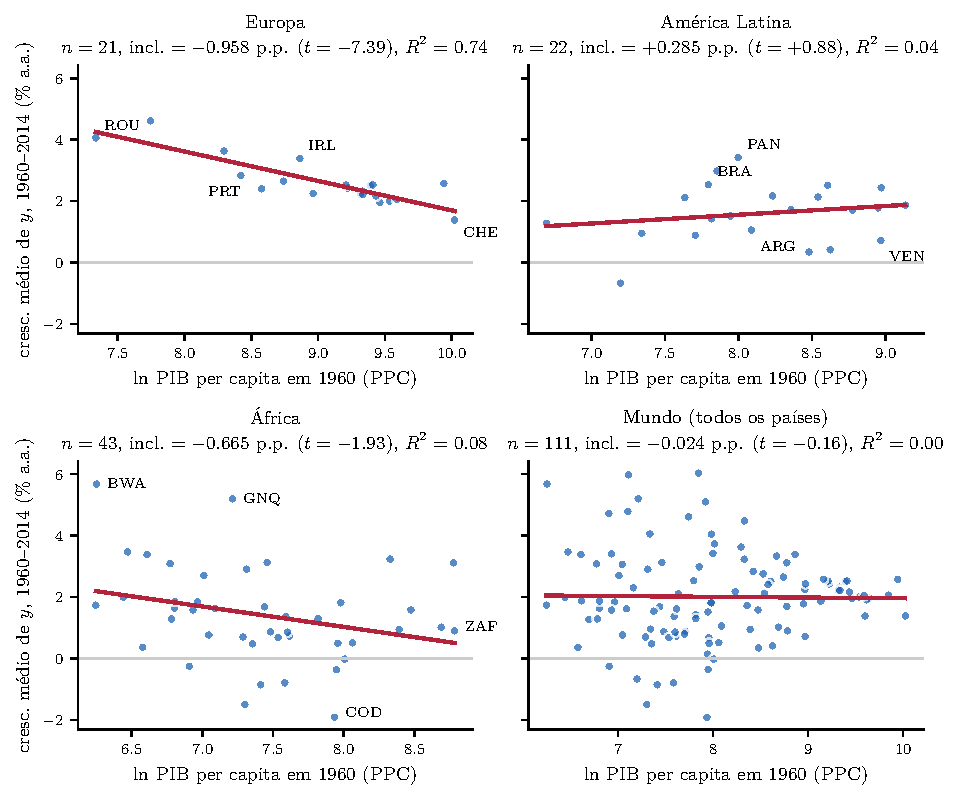
\includegraphics[width=\textwidth]{fig/fig_q3_convergencia.pdf}
\end{center}

\begin{center}
\small
\begin{tabular}{lrrrrl}
\toprule
\textbf{Região} & \textbf{$n$} & \textbf{Inclinação} & \textbf{(e.p.)} & \textbf{$t$} & \textbf{$R^2$} \\
\midrule
Europa           & 21  & $-0{,}00958$ & $(0{,}00130)$ & $-7{,}39$ & $0{,}742$ \\
América Latina   & 22  & $+0{,}00285$ & $(0{,}00325)$ & $+0{,}88$ & $0{,}037$ \\
África           & 43  & $-0{,}00665$ & $(0{,}00345)$ & $-1{,}93$ & $0{,}083$ \\
\midrule
Mundo (amostra toda) & 111 & $-0{,}00024$ & $(0{,}00151)$ & $-0{,}16$ & $0{,}000$ \\
\bottomrule
\end{tabular}
\end{center}

\resp{A resposta à pergunta é: sim, na Europa --- e de forma inequívoca. Não na América
Latina. Na África, não de forma robusta.}

\begin{itemize}
\item \textbf{Europa: convergência forte.} A inclinação de $-0{,}0096$ diz que um país
      $10\%$ mais pobre em 1960 cresceu cerca de $0{,}1$ ponto percentual ao ano a mais.
      Com $t = -7{,}4$ e $R^2 = 0{,}74$, o PIB per capita de 1960 sozinho explica três
      quartos da variação do crescimento em meio século. Romênia, Portugal, Grécia e
      Irlanda partiram muito atrás e fecharam boa parte do vão; Suíça, o país mais rico em
      1960 ($22{.}530$ dólares internacionais), cresceu a $1{,}38\%$ a.a., a menor taxa da
      região.

      \emph{Velocidade de convergência.} Cuidado ao converter a inclinação em velocidade:
      $b$ \textbf{não} é $-\lambda$. Regredindo o crescimento \emph{médio} de $T$ anos
      contra $\ln y_{1960}$, o Solow log-linearizado implica
      $b = -\left(1 - e^{-\lambda T}\right)/T$, ou seja
      $\lambda = -\ln(1 + bT)/T$. Com $T = 54$ e $b = -0{,}00958$ isso dá
      $\lambda = 1{,}35\%$ ao ano e \textbf{meia-vida do hiato de $\approx 51$ anos} ---
      próximo dos $2\%$ que a literatura de convergência costuma encontrar. A leitura
      ingênua $\lambda = -b = 0{,}96\%$ subestima a velocidade em um terço, porque ignora
      que a convergência já ocorreu \emph{durante} a janela de 54 anos.
\item \textbf{América Latina: nenhuma convergência.} A inclinação é \emph{positiva} e
      indistinguível de zero ($t = 0{,}88$, $R^2 = 0{,}04$). Ser pobre em 1960 não ajudou.
      A dispersão foi de crescimento negativo (Haiti, $-0{,}67\%$ a.a.) a mais de $3\%$
      (Panamá, $3{,}42\%$), com o Brasil em $2{,}54\%$ --- e essa dispersão não tem relação
      com o ponto de partida.
\item \textbf{África: negativa, mas frágil.} A $t = -1{,}93$ a inclinação mal escapa de
      zero, e $R^2 = 0{,}08$ significa que o nível inicial praticamente não prevê nada. O
      pouco que existe vem de dois casos de recursos naturais: Botsuana ($5{,}68\%$ a.a.,
      diamantes) e Guiné Equatorial ($5{,}20\%$, petróleo), ambos partindo de bases
      baixas. Retirando os dois, a inclinação encolhe para $-0{,}0038$ com $t = -1{,}23$ e
      $R^2 = 0{,}04$ --- \textbf{estatisticamente nada}. No outro extremo, R.D.\ do Congo
      ($-1{,}91\%$ a.a.) e República Centro-Africana ($-1{,}50\%$) \emph{empobreceram}
      durante 54 anos.
\item \textbf{Mundo: zero.} A inclinação é $-0{,}00024$ com $R^2$ de três casas
      zeradas --- a reta é horizontal. \textbf{Não há convergência absoluta na amostra
      mundial.} O quarto painel é a Figura 3.3.1 de Kurlat, e serve de referência contra a
      qual ler os outros três.
\end{itemize}

\passo{Passo 3 --- Uma segunda evidência, independente: $\sigma$-convergência.} A
inclinação mede $\beta$-convergência (pobres crescem mais). A pergunta complementar é se a
\emph{dispersão} de renda diminuiu. Comparando o desvio-padrão de $\ln y$ nas duas pontas:

\begin{center}
\small
\begin{tabular}{lccl}
\toprule
\textbf{Região} & \textbf{d.p.\ de $\ln y$, 1960} & \textbf{2014} & \\
\midrule
Europa         & $0{,}674$ & $0{,}391$ & $\sigma$-convergência \\
América Latina & $0{,}640$ & $0{,}889$ & $\sigma$-divergência \\
África         & $0{,}675$ & $0{,}905$ & $\sigma$-divergência \\
\bottomrule
\end{tabular}
\end{center}

As três regiões partiram de dispersões quase idênticas em 1960. A Europa comprimiu a sua
em $42\%$; América Latina e África \textbf{aumentaram} a delas em cerca de $40\%$. Os dois
critérios concordam, o que dá bastante confiança à leitura. \checkmark

\passo{Passo 4 --- Interpretação: é a distinção entre convergência absoluta e
condicional.} O exercício é construído para produzir exatamente este ponto --- \emph{a
amostra mundial não converge, mas uma sub-amostra pode}.

Solow prevê que cada país converge para o \textbf{seu próprio} estado estacionário
$$k\stst = \left(\frac{s}{n+\delta}\right)^{\frac{1}{1-\alpha}},$$
que depende de $s$, $n$, $\delta$ e da tecnologia daquele país. Isso é
\textbf{convergência condicional}: cada um se aproxima do \emph{seu} alvo, tão mais rápido
quanto mais longe estiver dele. Só vira convergência \textbf{absoluta} se todos
compartilharem o mesmo alvo.

\begin{itemize}
\item Na \textbf{Europa} --- instituições parecidas, taxas de poupança e demografia
      parecidas, livre circulação de capital, tecnologia e trabalho, e para vários o efeito
      disciplinador da adesão à UE --- supor um estado estacionário \emph{comum} é
      defensável. Aí a convergência condicional aparece \emph{como se} fosse absoluta. Note
      que retirar a Romênia (único ex-socialista com dado de 1960) até fortalece o
      resultado: inclinação $-0{,}0102$, $t = -6{,}26$. O efeito não é um artefato da
      transição pós-1990.
\item Na \textbf{África}, os estados estacionários diferem enormemente: instituições,
      conflito armado, saúde, escolaridade, geografia e política variam muito mais do que a
      renda inicial. Os países estão convergindo --- para alvos radicalmente diferentes. Um
      gráfico contra a renda inicial, sozinho, não tem como enxergar isso.
\end{itemize}

É o fenômeno dos \textbf{clubes de convergência}: grupos homogêneos convergem
internamente; o mundo, como um todo, não.

\passo{Passo 5 --- Duas ressalvas que valem ponto.}

\emph{(i) Recortar por região não é o mesmo que controlar por $s$ e $n$.} A região é uma
proxy grosseira e observável para ``ter o mesmo estado estacionário''. O teste próprio de
convergência condicional estima
$$g_i = \beta_0 + \beta_1 \ln y_{i,1960} + \beta_2 \ln s_i
      + \beta_3 \ln(n_i + g + \delta) + \varepsilon_i$$
e pergunta se $\beta_1 < 0$. Feito assim, $\beta_1$ é negativo até na amostra mundial ---
o que é precisamente a afirmação de que a convergência é condicional. O recorte regional é
a versão transparente e sem regressão desse teste.

\emph{(ii) Seleção amostral.} Exigir dado em 1960 \emph{e} em 2014 descarta justamente os
países cujos sistemas estatísticos desmoronaram --- que tendem a ser os piores
desempenhos. Isso enviesa o crescimento africano \textbf{para cima} e subestima a
divergência. A amostra africana aqui tem 43 países, o que é bom para a PWT, mas os
ausentes não são ausentes ao acaso.

\intuicao{Produtividade marginal decrescente do capital é o motor da convergência: quem
tem pouco capital por trabalhador tem retorno alto e, com a mesma taxa de poupança,
cresce mais rápido. Mas ``a mesma taxa de poupança'' é hipótese, não fato. O que os
gráficos mostram é que essa hipótese é razoável dentro da Europa e insustentável dentro da
África. Solow não erra na África --- ele simplesmente não prevê o que muita gente acha que
prevê. A força do exercício é ver os dois casos lado a lado, com a mesma metodologia e a
mesma base.}

\refbib{Kurlat (2020), §3.3 ``Growth Across Countries'' (p.\ 51) e a Figura 3.3.1;
enunciado do Exercício 3.3 na p.\ 51. A interpretação via estados estacionários distintos
antecipa §4.2 ``Mechanics'' (p.\ 57), e a evidência quantitativa reaparece em §5.3.
Complementar: Jones (2020, 5\textordfeminine{} ed.), cap.\ 3, para os mesmos gráficos com
exposição mais visual. Dados: Feenstra, Inklaar \& Timmer (2015), \emph{Penn World Table
10.01}.}

\begin{tcolorbox}[rubricbox]
\small
\textbf{2,0 pontos:} três diagramas com eixos rotulados e reta ajustada (0,8 --- eixos,
escala log no nível inicial e a reta pontuam separadamente); leitura correta do sinal em
cada região (0,4); resposta explícita à pergunta ``em alguma região os pobres cresceram
mais rápido?'' (0,3); interpretação via convergência \textbf{condicional} vs.\
\textbf{absoluta} (0,5).

\smallskip
\textbf{Tetos por erro conceitual:}
\begin{itemize}[topsep=2pt]
\item Concluir que ``Solow está errado'' porque a África não converge: máx.\ 1,0. O modelo
      prevê convergência \emph{condicional}.
\item Usar média aritmética das taxas anuais em vez da geométrica: $-0{,}3$.
\item Entregar os gráficos sem reta ajustada nem inclinação: máx.\ 1,2 --- a pergunta é
      sobre sinal e magnitude.
\item Não apresentar gráfico algum, apenas texto: máx.\ 0,8.
\end{itemize}
\textbf{Bônus:} trazer $\sigma$-convergência como segunda evidência, ou notar o viés de
seleção da amostra.

\smallskip
\textbf{Risco residual:} a composição da lista de países muda os números. Declare quais
países entraram em cada região --- duas respostas corretas podem divergir na terceira casa
decimal e ambas estarem certas.
\end{tcolorbox}

%======================================================================
\section[Questão 4 --- Terremoto no modelo de Solow]{Questão 4 \quad Terremoto no modelo de Solow \hfill \normalsize (3 pontos)}
%======================================================================

\begin{tcolorbox}[questionbox]
\small
Baseado em Kurlat (2020, Cap.\ 4). Uma economia se comporta de acordo com o modelo de
crescimento de Solow. Ela começa em $t=0$ em estado estacionário, \textbf{sem progresso
tecnológico}. Um terremoto ocorre em $t = t_0$, destruindo \textbf{metade do estoque de
capital}.

\textbf{(a)} O que aconteceria, no curto prazo e no longo prazo, com o PIB e o PIB per
capita?

\textbf{(b)} Suponha agora que, além da destruição do capital, a taxa de crescimento
populacional seja \textbf{reduzida à metade}, pois as pessoas passam a emigrar. Como os
efeitos sobre o PIB e o PIB per capita mudam nesse caso?
\end{tcolorbox}

\passo{Montagem.} Produção com retornos constantes de escala, Cobb--Douglas para fixar
ideias:
$$Y_t = F(K_t, L_t) = K_t^{\alpha} L_t^{1-\alpha}, \qquad 0<\alpha<1 .$$
Em termos \textbf{por trabalhador} --- e é preciso declarar isso, porque sem progresso
tecnológico ``por trabalhador'' e ``por unidade de eficiência'' coincidem, mas o hábito de
declarar evita ambiguidade nas questões da Aula 3 ---, com $k \equiv K/L$ e $y \equiv Y/L$:
$$y = f(k) = k^{\alpha}, \qquad
\dot k = s f(k) - (n+\delta)k .$$
O estado estacionário resolve $s f(k\stst) = (n+\delta) k\stst$, ou seja
$$k\stst = \left(\frac{s}{n+\delta}\right)^{\frac{1}{1-\alpha}}, \qquad
y\stst = \left(\frac{s}{n+\delta}\right)^{\frac{\alpha}{1-\alpha}} .$$

\textbf{Note o que $k\stst$ contém, porque é a chave dos dois itens:} apenas
$s$, $n$, $\delta$ e $\alpha$. \textbf{O nível de $k$ não aparece.} O estado estacionário é
um atrator determinado por parâmetros; de onde a economia parte não altera para onde ela
vai. Toda a questão decorre disso.

Calibração ilustrativa usada nos gráficos e nos números: $\alpha = 1/3$, $s = 0{,}20$,
$\delta = 0{,}05$, $n = 0{,}02$.

%---------------------------------------------------------------- (a)
\subsection*{(a) Terremoto: destruição de metade do capital}

\passo{Passo 1 --- O impacto.} O terremoto destrói capital, não pessoas. Logo $L$ não muda
e
$$K_{t_0} \to \tfrac{1}{2}K_{t_0} \;\Longrightarrow\; k_{t_0} \to \tfrac{1}{2}k\stst .$$
O produto por trabalhador cai imediatamente, mas \textbf{menos que proporcionalmente}:
$$\frac{y_{t_0}}{y\stst} = \left(\frac{k\stst/2}{k\stst}\right)^{\alpha} = 2^{-\alpha}
= 2^{-1/3} = 0{,}794
\;\Longrightarrow\; \resp{-20{,}6\%} .$$
Metade do capital some e o PIB per capita cai um quinto --- é a participação do capital
$\alpha$ amortecendo o golpe. Como $L$ está intacto, o PIB agregado
$Y = y \cdot L$ cai exatamente na mesma proporção, $-20{,}6\%$.

\passo{Passo 2 --- O curto prazo: a economia cresce, e cresce rápido.} Em
$k = k\stst/2 < k\stst$, o investimento efetivo supera o de reposição:
$$\frac{\dot k}{k} = s k^{\alpha-1} - (n+\delta)
\;\Big|_{\,k = k\stst/2} = (n+\delta)\left(2^{1-\alpha} - 1\right) > 0 .$$
Com a calibração: $(0{,}07)(2^{2/3}-1) = 4{,}11\%$ ao ano para $k$, e como
$\dot y/y = \alpha\,\dot k/k$, o PIB per capita cresce a $1{,}37\%$ ao ano logo após o
choque --- contra $0\%$ antes dele. O PIB agregado cresce a $n + 1{,}37\% = 3{,}37\%$
ao ano.

Essa taxa \textbf{decai monotonicamente} à medida que $k$ sobe: é o retorno marginal
decrescente do capital. Na simulação, metade do hiato de $y$ se fecha em $13$ anos, $90\%$
em $46$ anos e $99\%$ em $94$ anos. A recuperação é rápida no começo e lenta na cauda.

\passo{Passo 3 --- O longo prazo: nada mudou.} Como $s$, $n$, $\delta$ e $\alpha$ estão
todos intactos, $k\stst$ é o mesmo de antes. A economia volta a
$$k \to k\stst, \qquad y \to y\stst,$$
\textbf{exatamente os valores anteriores ao terremoto}. E como a trajetória de $L$ também
não foi tocada, o PIB agregado retorna à \emph{mesma trajetória} $Y_t = y\stst L_0 e^{nt}$
que teria seguido sem o terremoto --- não a uma trajetória paralela abaixo, mas à original.
Na simulação, $Y/Y^{\text{contrafactual}} = 1{,}0000$ ao fim do horizonte. \checkmark

\begin{center}
\begin{tikzpicture}
\begin{axis}[
  width=9.2cm, height=6.2cm,
  xlabel={$k$}, ylabel={por trabalhador},
  xmin=0, xmax=8.2, ymin=0, ymax=0.62,
  axis lines=left, xtick={2.415, 4.83}, xticklabels={$k\stst/2$, $k\stst$},
  ytick=\empty, legend style={at={(0.98,0.30)}, anchor=east, draw=none,
  fill=none, font=\small}, clip=false,
]
\addplot[domain=0.01:8.2, samples=200, thick, darkblue] {0.20*x^(1/3)};
\addlegendentry{$s\,f(k)$}
\addplot[domain=0:8.2, samples=2, thick, evencolor] {0.07*x};
\addlegendentry{$(n+\delta)k$}
\draw[dashed, gray] (axis cs:4.83,0) -- (axis cs:4.83,0.3381);
\draw[dashed, gray] (axis cs:2.415,0) -- (axis cs:2.415,0.2684);
% seta do choque
\draw[-{Stealth[length=3mm]}, red!70!black, very thick]
  (axis cs:4.83,0.045) -- node[above, font=\scriptsize, pos=0.5] {terremoto} (axis cs:2.415,0.045);
% setas de retorno (escritas uma a uma: \foreach nao sobrevive ao adiamento
% do desenho dentro do ambiente axis)
\draw[-{Stealth[length=2mm]}, darkblue] (axis cs:2.70,0.015) -- (axis cs:3.15,0.015);
\draw[-{Stealth[length=2mm]}, darkblue] (axis cs:3.30,0.015) -- (axis cs:3.75,0.015);
\draw[-{Stealth[length=2mm]}, darkblue] (axis cs:3.90,0.015) -- (axis cs:4.35,0.015);
% rotulo na regiao em que a desigualdade de fato vale: a ESQUERDA de k*
\node[font=\scriptsize, darkblue, align=center] at (axis cs:2.05,0.52)
  {$s f(k) > (n+\delta)k$\\[-1pt] $\Rightarrow\ \dot k > 0$};
\end{axis}
\end{tikzpicture}
\end{center}

\resp{Resposta de (a): no curto prazo, PIB e PIB per capita caem $\bm{20{,}6\%}$ (isto é,
$1-2^{-\alpha}$) e em seguida crescem a taxas positivas e decrescentes. No longo prazo,
ambos retornam \emph{exatamente} à trajetória original --- o PIB per capita ao mesmo nível
$y\stst$, o PIB agregado à mesma senda de crescimento à taxa $n$. O terremoto não tem
efeito permanente.}

\intuicao{Um choque no \emph{estoque} de capital é transitório porque $k\stst$ depende de
\emph{fluxos} (a taxa de poupança, a de depreciação, a demográfica), não do nível herdado
de capital. E a recuperação é rápida justamente porque o capital ficou escasso: com
$k$ pela metade, a produtividade marginal do capital é $2^{1-\alpha} = 1{,}59$ vezes a
normal, o investimento rende muito, e a economia se reconstrói sozinha. É a mesma mecânica
que explica o crescimento acelerado de Alemanha e Japão no pós-guerra --- não um milagre
de política, mas o modelo de Solow funcionando como previsto. Um leitor que confunda o
choque de $K$ com um choque em $s$ erra a questão inteira: só o segundo desloca $k\stst$.}

%---------------------------------------------------------------- (b)
\subsection*{(b) Terremoto \emph{mais} queda de $n$ pela metade}

Agora, além de $k_{t_0} \to k\stst/2$, a taxa de crescimento populacional cai
permanentemente de $n$ para $n/2$ a partir de $t_0$.

\begin{tcolorbox}[theorybox, title={Leitura do enunciado --- declare a sua}]
\small
O enunciado diz que a \emph{taxa de crescimento} populacional cai à metade, não que a
população cai à metade. Resolvo assim: $n' = n/2$ de $t_0$ em diante, com $L_{t_0}$
inalterado. \textbf{Uma emigração realista também produziria um salto de nível em $L$},
que \emph{elevaria} $k = K/L$ no impacto e amorteceria parte da queda de $y$ --- efeito
transitório, que não altera nada do que se segue sobre o longo prazo. Como o enunciado é
ambíguo nesse ponto, o certo é declarar a leitura adotada.
\end{tcolorbox}

\passo{Passo 1 --- O impacto é o mesmo.} Em $t_0$, $L$ ainda não mudou (só sua taxa de
crescimento futura mudou), então a queda instantânea de $y$ e de $Y$ é de novo
$-20{,}6\%$. A diferença entre (a) e (b) está toda no que vem depois.

\passo{Passo 2 --- O alvo se desloca para cima.} A reta de reposição
$(n+\delta)k$ \textbf{gira para baixo}, tornando-se $(n/2+\delta)k$: é preciso menos
investimento por trabalhador para manter $k$ constante, porque há menos trabalhadores
novos para equipar a cada ano. O novo estado estacionário é
$$k\ststst = \left(\frac{s}{n/2+\delta}\right)^{\frac{1}{1-\alpha}} > k\stst,
\qquad
\frac{y\ststst}{y\stst}
= \left(\frac{n+\delta}{n/2+\delta}\right)^{\frac{\alpha}{1-\alpha}} .$$
Com a calibração: $k\stst = 4{,}83 \to k\ststst = 6{,}09$ e
$y\ststst/y\stst = (0{,}07/0{,}06)^{1/2} = 1{,}0801$, isto é, \resp{$+8{,}0\%$
permanentes} no PIB per capita. A simulação numérica devolve $1{,}0801$. \checkmark

\begin{center}
\begin{tikzpicture}
\begin{axis}[
  width=9.2cm, height=6.2cm,
  xlabel={$k$}, ylabel={por trabalhador},
  xmin=0, xmax=8.2, ymin=0, ymax=0.62,
  axis lines=left, xtick={2.415, 4.83, 6.086},
  xticklabels={$k\stst/2$, $k\stst$, $k\ststst$},
  ytick=\empty, legend style={at={(0.99,0.32)}, anchor=east, draw=none,
  fill=none, font=\small}, clip=false,
]
\addplot[domain=0.01:8.2, samples=200, thick, darkblue] {0.20*x^(1/3)};
\addlegendentry{$s\,f(k)$}
\addplot[domain=0:8.2, samples=2, thick, evencolor, dashed] {0.07*x};
\addlegendentry{$(n+\delta)k$}
\addplot[domain=0:8.2, samples=2, thick, red!70!black] {0.06*x};
\addlegendentry{$(n/2+\delta)k$}
\draw[dashed, gray] (axis cs:4.83,0) -- (axis cs:4.83,0.3381);
\draw[dashed, gray] (axis cs:6.086,0) -- (axis cs:6.086,0.3652);
\draw[dashed, gray] (axis cs:2.415,0) -- (axis cs:2.415,0.2684);
\draw[-{Stealth[length=3mm]}, red!70!black, very thick]
  (axis cs:4.83,0.045) -- node[above, font=\scriptsize] {terremoto} (axis cs:2.415,0.045);
\draw[-{Stealth[length=2mm]}, red!70!black] (axis cs:2.70,0.015) -- (axis cs:3.25,0.015);
\draw[-{Stealth[length=2mm]}, red!70!black] (axis cs:3.50,0.015) -- (axis cs:4.05,0.015);
\draw[-{Stealth[length=2mm]}, red!70!black] (axis cs:4.30,0.015) -- (axis cs:4.85,0.015);
\draw[-{Stealth[length=2mm]}, red!70!black] (axis cs:5.10,0.015) -- (axis cs:5.65,0.015);
% canto superior esquerdo: unica area livre (a direita fica a legenda)
\node[font=\scriptsize, red!70!black, align=center] at (axis cs:2.05,0.52)
  {reta de reposição gira\\[-1pt] para baixo: $k\ststst > k\stst$};
\end{axis}
\end{tikzpicture}
\end{center}

\passo{Passo 3 --- A transição é mais rápida.} O hiato a fechar é maior ($k\stst/2$ até
$k\ststst$, em vez de até $k\stst$), então a taxa de crescimento inicial é maior:
$5{,}11\%$ ao ano para $k$ e $1{,}70\%$ para $y$, contra $4{,}11\%$ e $1{,}37\%$ em (a).
Na simulação, $y$ recupera o \emph{antigo} nível $y\stst$ cerca de $30$ anos depois do
choque --- e continua subindo até $y\ststst$.

\passo{Passo 4 --- O ponto decisivo: PIB per capita e PIB agregado divergem.}

\begin{itemize}
\item \textbf{PIB per capita: permanentemente MAIOR.} $y \to y\ststst = 1{,}080\,y\stst$.
      O país acaba mais rico por pessoa \emph{do que era antes do terremoto}. Menos gente
      nova para equipar significa mais capital por trabalhador --- é o efeito de
      \textbf{diluição de capital}, com o sinal invertido.
\item \textbf{PIB agregado: permanentemente MENOR que o contrafactual, e afastando-se sem
      limite.} $Y_t = y_t L_t$, e agora $L_t$ cresce a $n/2$ em vez de $n$. Comparando com
      a trajetória sem terremoto,
      $$\frac{Y_t}{Y_t^{\text{contra}}} \;\longrightarrow\;
      \frac{y\ststst}{y\stst}\; e^{-\frac{n}{2}(t - t_0)} \;\longrightarrow\; 0 .$$
      O ganho de $8\%$ no numerador é um fator constante; o denominador cresce
      exponencialmente. Na simulação, ao fim de 200 anos após o choque o PIB agregado é
      $15\%$ do contrafactual --- e a razão continua caindo para sempre.
\item \textbf{Taxas de crescimento de longo prazo.} $y$ volta a crescer a $0\%$ (não há
      progresso tecnológico --- este é o resultado central da Aula 2, e ele sobrevive
      intacto). $Y$ passa a crescer a $n/2$ em vez de $n$: mais lento, permanentemente.
\end{itemize}

\begin{center}
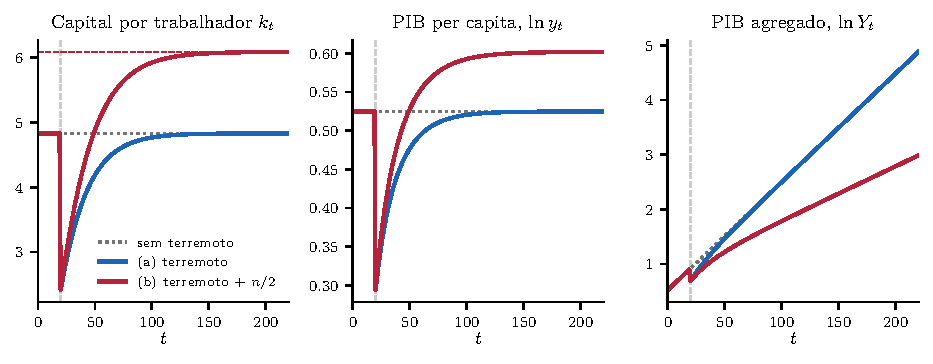
\includegraphics[width=\textwidth]{fig/fig_q4_trajetorias.pdf}
\end{center}

\passo{Passo 5 --- E o bem-estar?} Como $s$ é fixa, o consumo por trabalhador em estado
estacionário é $c\stst = (1-s) f(k\stst)$, que é \textbf{crescente em $k\stst$ sem
ressalva}. Logo $c\ststst > c\stst$: o consumo per capita também sobe $8\%$.

Vale ser explícito sobre uma armadilha aqui: \emph{não} é caso de invocar a Regra de Ouro
e perguntar se a economia passou do ponto. A Regra de Ouro trata da escolha de $s$ dado
$(n+\delta)$; aqui $s$ está fixa e o que mudou foi $n$. Com $s$ constante,
$c\stst = (1-s)f(k\stst)$ sobe sempre que $k\stst$ sobe --- não há trade-off. (Confira a
consistência: em estado estacionário $f(k\stst) - (n+\delta)k\stst = (1-s)f(k\stst)$, pois
$(n+\delta)k\stst = sf(k\stst)$. \checkmark)

\resp{Resposta de (b): o impacto de curto prazo é o mesmo ($-20{,}6\%$), mas a
recuperação é mais rápida e vai além. O PIB per capita ultrapassa o nível anterior e se
estabiliza $8\%$ acima dele --- permanentemente maior. O PIB agregado, ao contrário, fica
permanentemente abaixo da trajetória que teria seguido, e a distância cresce sem limite,
porque a população passa a crescer a $n/2$. Nenhuma das duas variáveis tem crescimento de
longo prazo por pessoa: $g_y = 0$ como antes, e $g_Y$ cai de $n$ para $n/2$.}

\intuicao{Os dois itens juntos separam três coisas que se confundem com facilidade:
\textbf{nível} $\times$ \textbf{taxa}, e \textbf{agregado} $\times$ \textbf{per capita}.
O terremoto sozinho é puro transitório --- não mexe em nenhum parâmetro, então não mexe em
nada de permanente. A queda de $n$ mexe num parâmetro, e por isso desloca o nível de
longo prazo de $y$ --- mas ainda assim \emph{não} gera crescimento de longo prazo, apenas
um patamar mais alto alcançado durante a transição. E o mesmo choque tem sinais opostos
nas duas medidas de PIB: bom para quem fica, ruim para o tamanho da economia. Um país que
esvazia pode perfeitamente enriquecer por pessoa; a experiência da Europa pós-Peste Negra
é o exemplo histórico clássico, e é exatamente esta mecânica.}

\refbib{Kurlat (2020), §4.1 ``Ingredients of the Model'' (p.\ 53) e §4.2 ``Mechanics''
(pp.\ 57--60) --- diagrama de Solow, estabilidade e estática comparativa de $n$; enunciado
dos exercícios do cap.\ 4 na p.\ 72. Para o tratamento formal da dinâmica de transição e da
velocidade de convergência, Romer (2012, 4\textordfeminine{} ed.), cap.\ 1, §1.3--1.5.
Cuidado: §4.3 (Regra de Ouro) pertence à Aula 3 e \textbf{não} é necessária aqui.}

\begin{tcolorbox}[rubricbox]
\small
\textbf{(a)} 1,5 --- queda no impacto com o sinal e a lógica corretos, $y$ cai menos que
$K$ (0,4); crescimento positivo e decrescente na transição, com diagrama de Solow
rotulado (0,5 --- eixos, curvas nomeadas e direção do movimento pontuam separadamente da
conclusão verbal); retorno ao \emph{mesmo} $y\stst$ e à \emph{mesma} trajetória de $Y$,
justificado por $k\stst$ não depender de $k_0$ (0,6).

\smallskip
\textbf{(b)} 1,5 --- rotação da reta de reposição e novo $k\ststst > k\stst$ (0,5);
$y$ permanentemente \textbf{maior} (0,5); $Y$ permanentemente \textbf{menor} que o
contrafactual, crescendo a $n/2$ (0,5).

\smallskip
\textbf{Tetos por erro conceitual:}
\begin{itemize}[topsep=2pt]
\item Afirmar que o terremoto reduz o PIB per capita \emph{permanentemente} em (a):
      máx.\ 0,5 no item --- é o erro central da questão.
\item Tratar a queda de $n$ como se gerasse crescimento de longo prazo de $y$ (efeito de
      taxa em vez de efeito de nível): máx.\ 0,7 em (b).
\item Não distinguir PIB agregado de PIB per capita em (b), dando uma resposta só:
      máx.\ 0,8 em (b) --- a questão pergunta pelos dois, e eles têm sinais opostos.
\item Escrever a reta de reposição como $\delta k$, esquecendo $n$: máx.\ 0,8 na questão.
\item Usar $\Delta k = s f(k)$ sem depreciação: máx.\ 0,5 na questão.
\item Invocar a Regra de Ouro para dizer que o ganho de (b) é ambíguo: $-0{,}3$ ---
      com $s$ fixa, $c\stst$ sobe sem ambiguidade.
\end{itemize}
\textbf{Penalidade leve:} erro aritmético com método correto, $-0{,}2$ (não cumulativo com
os tetos acima).

\smallskip
\textbf{Risco residual:} o enunciado não diz se a emigração derruba o \emph{nível} de $L$
além da taxa. Declarar a leitura adotada protege a resposta; não declarar deixa a solução
ambígua num ponto que muda a magnitude da queda no impacto.
\end{tcolorbox}

%======================================================================
\section*{Síntese --- o fio que liga as quatro questões}
\addcontentsline{toc}{section}{Síntese}
%======================================================================

\begin{tcolorbox}[theorybox, title={O que a Lista 1 está realmente testando}]
\small
\begin{itemize}
\item \textbf{Q1} --- um agregado macro só tem sentido depois que se declara o vetor de
      preços. Laspeyres e Paasche delimitam uma faixa; Fisher é a convenção. O mesmo
      problema, no tempo (itens b--c) e no espaço (itens d--e).
\item \textbf{Q2} --- o PIB é uma medida incompleta \emph{e} corrigível: preferência
      revelada transforma ``o que falta'' em peso estimável.
\item \textbf{Q3} --- Solow prevê convergência \textbf{condicional}. A Europa parece
      convergir em termos absolutos porque seus estados estacionários são parecidos; o
      mundo não converge porque os dele não são.
\item \textbf{Q4} --- \emph{nível} não é \emph{taxa}, e \emph{agregado} não é
      \emph{per capita}. Choque em estoque é transitório; choque em parâmetro desloca o
      nível de longo prazo; e nenhum dos dois gera crescimento sustentado de $y$ sem
      progresso tecnológico.
\end{itemize}
As três armadilhas com maior peso somado na lista são: (i) achar que uma das taxas de
crescimento da Q1 está errada; (ii) concluir da Q3 que Solow foi refutado; (iii) atribuir
efeito permanente ao terremoto na Q4(a). Juntas, valem cerca de 3 pontos.
\end{tcolorbox}

%======================================================================
\section*{Apêndice \quad Código}
\addcontentsline{toc}{section}{Apêndice --- Código}
%======================================================================

Os scripts estão em \texttt{Resolucao/lista1\_codigo/} e rodam com \texttt{numpy},
\texttt{pandas} e \texttt{matplotlib}. O módulo \texttt{estilo\_mpl.py} força o backend
\texttt{pgf}, para que o texto das figuras seja composto pelo próprio pdf\LaTeX{} em fontes
Type 1 --- sem ele o matplotlib embute DejaVu como Type 3 e o texto do PDF deixa de ser
copiável.

\begin{center}
\small
\begin{tabular}{llp{7.4cm}}
\toprule
\textbf{Arquivo} & \textbf{Questão} & \textbf{O que faz} \\
\midrule
\texttt{q1\_pib.py}         & 1 & Todos os números da Q1 em aritmética exata de frações;
  índices de Laspeyres, Paasche e Fisher; decomposição de Bortkiewicz; câmbio PPC
  implícito. Inclui os testes de consistência marcados \checkmark. \\
\texttt{q3\_convergencia.py}& 3 & Monta o painel da PWT 10.01, calcula $g_i$ e
  $\ln y_{i,1960}$, roda as regressões por região com erro-padrão e $R^2$, e reporta
  extremos e $\sigma$-convergência. \\
\texttt{q3\_figura.py}      & 3 & Gera \texttt{fig\_q3\_convergencia.pdf} --- os três
  diagramas pedidos mais o painel do mundo. \\
\texttt{q4\_solow.py}       & 4 & Simula o Solow em tempo discreto nos dois cenários mais o
  contrafactual; confere as fórmulas analíticas contra a simulação; gera
  \texttt{fig\_q4\_trajetorias.pdf}. \\
\texttt{estilo\_mpl.py}     & 3, 4 & Backend \texttt{pgf} e tamanho das figuras casado com
  a largura do texto (sem reescalonamento). Importado pelos dois scripts de figura. \\
\bottomrule
\end{tabular}
\end{center}

\passo{Reprodução.} A PWT não está versionada no repositório (6,5\,MB). Baixe-a antes de
rodar os scripts da Q3:

\begin{tcolorbox}[colback=gray!7, colframe=gray!50, arc=2pt, boxrule=0.4pt]
\footnotesize
\begin{verbatim}
curl -L -o pwt1001.xlsx https://dataverse.nl/api/access/datafile/354095
python q3_convergencia.py    # tabela de regressoes
python q3_figura.py          # fig_q3_convergencia.pdf
python q1_pib.py             # numeros da Questao 1
python q4_solow.py           # numeros e figura da Questao 4
\end{verbatim}
\end{tcolorbox}

\vspace{4pt}
{\small\textcolor{gray!60!black}{\textbf{Fonte dos dados:} Feenstra, Robert C., Robert
Inklaar \& Marcel P.\ Timmer (2015), ``The Next Generation of the Penn World Table'',
\emph{American Economic Review} 105(10), 3150--3182. Versão 10.01, disponível em
\url{www.ggdc.net/pwt}.}}

\end{document}
